\documentclass{article}
\usepackage{placeins}
\usepackage{graphicx}
\usepackage{subcaption}
\usepackage{listings}
\usepackage{cleveref}
\usepackage{booktabs, siunitx}
\usepackage[svgnames,table]{xcolor}
\usepackage[utf8]{inputenc}
\usepackage{geometry}

\geometry{
 a4paper,
 total={170mm,257mm},
 left=20mm,
 top=20mm,
 }
\graphicspath{ {./images/} }

\title{Assignment 1 Report}
\author{Tanat Tangun}
\date{August 2022}

\begin{document}
\maketitle
\section{Flood Dataset}
\subsection*{Problem}
We want to predict water level at 7 hours ahead given station 1 and station 2 data at present and 3 hours before.
\begin{figure}[ht]
	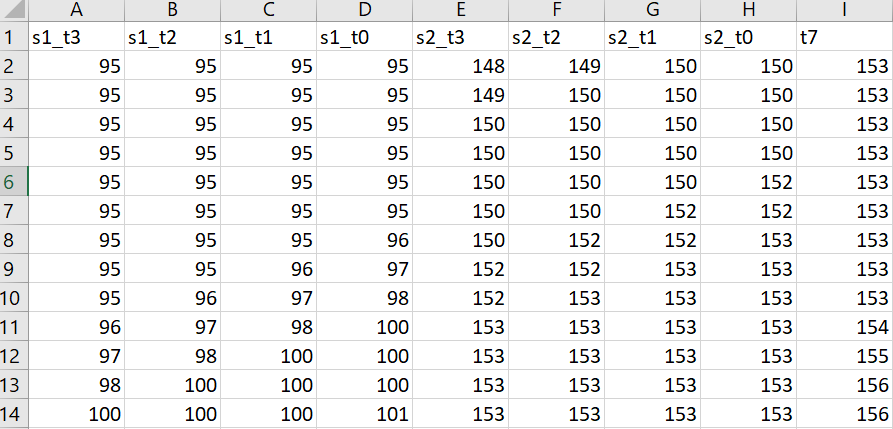
\includegraphics[width=\textwidth]{flood_data}
	\caption{Examples of given data
		where s1\_t3 is a water level from 3 hours before at station 1, t7 is water level at 7 hours ahead, and so on.}
	\centering
\end{figure}

\subsection*{Parameters Setting}
\begin{itemize}
	\item All nodes use $sigmoid$ as an activation function except output node that use $linear$ function.
	\item Weights is a random number between $[-1, 1]$
	\item Each layer's bias is $1$
	\item Use MSE (Mean Squared Error) as a loss function.
\end{itemize}

\subsection*{Training}
Use 10\% cross-validation, and preprocess our data by using training set $mean$ and $std$ to standardize (For each data point $x$ we calculate new $x' = \frac{x - mean}{std}$) both training set and validation set before training with SGD (Stochastic Gradient Descent) algorithm. Then, we train each cross-validation set for $1000$ epochs.
\\ \\
We will create one base network that should perform good enough and create a variation base on that network, that is train with no \emph{momentum}, train with smaller \emph{learning rate}, and add more layers or hidden nodes to see that if we introduce those variations, will the network perform better, converge faster or no improvement at all?

\subsection*{Training Result}
\subsubsection*{Flood-8-4-1}
Our base network that contains only 8 input nodes, 1 hidden layer with 4 nodes, and 1 output node train with $lr = 0.01$ and $momentum = 0.01$.
\\ \\
Below is the graphs we get from training this network. The training process take about $60$ seconds.
\begin{figure}[ht]
	\begin{subfigure}{\textwidth}
		\centering
		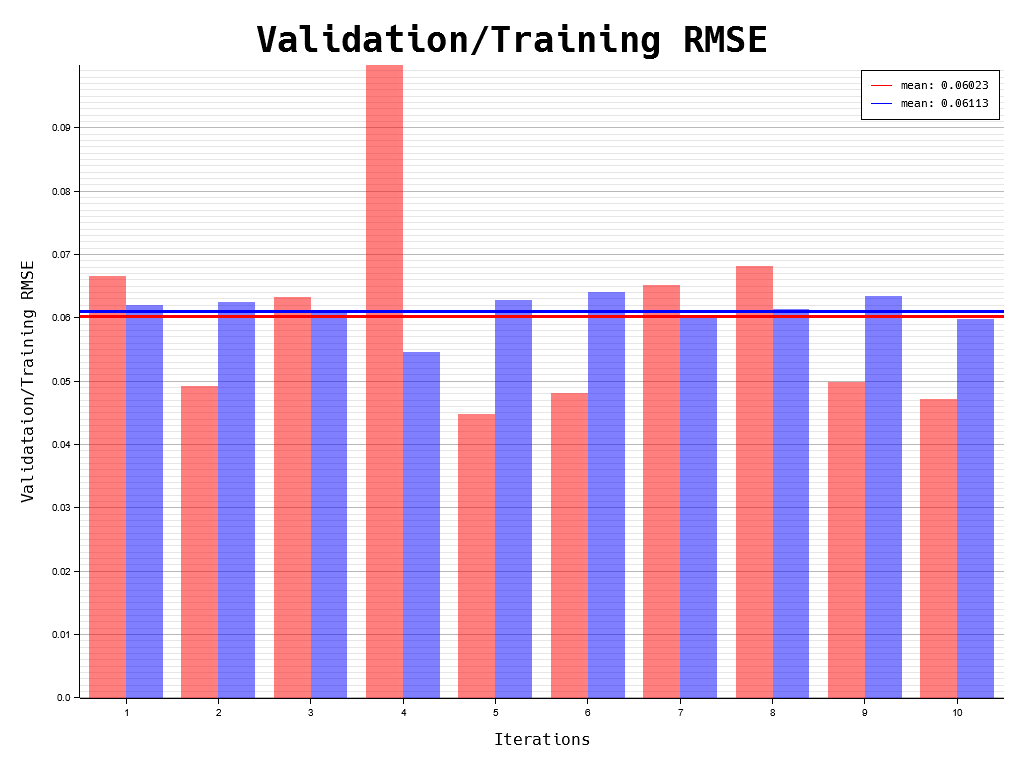
\includegraphics[scale=0.3]{flood-8-4-1/cv_l}
		\caption{Each iteration training (blue) and validation (red) MSE at last epoch}
	\end{subfigure}
	\begin{subfigure}{\textwidth}
		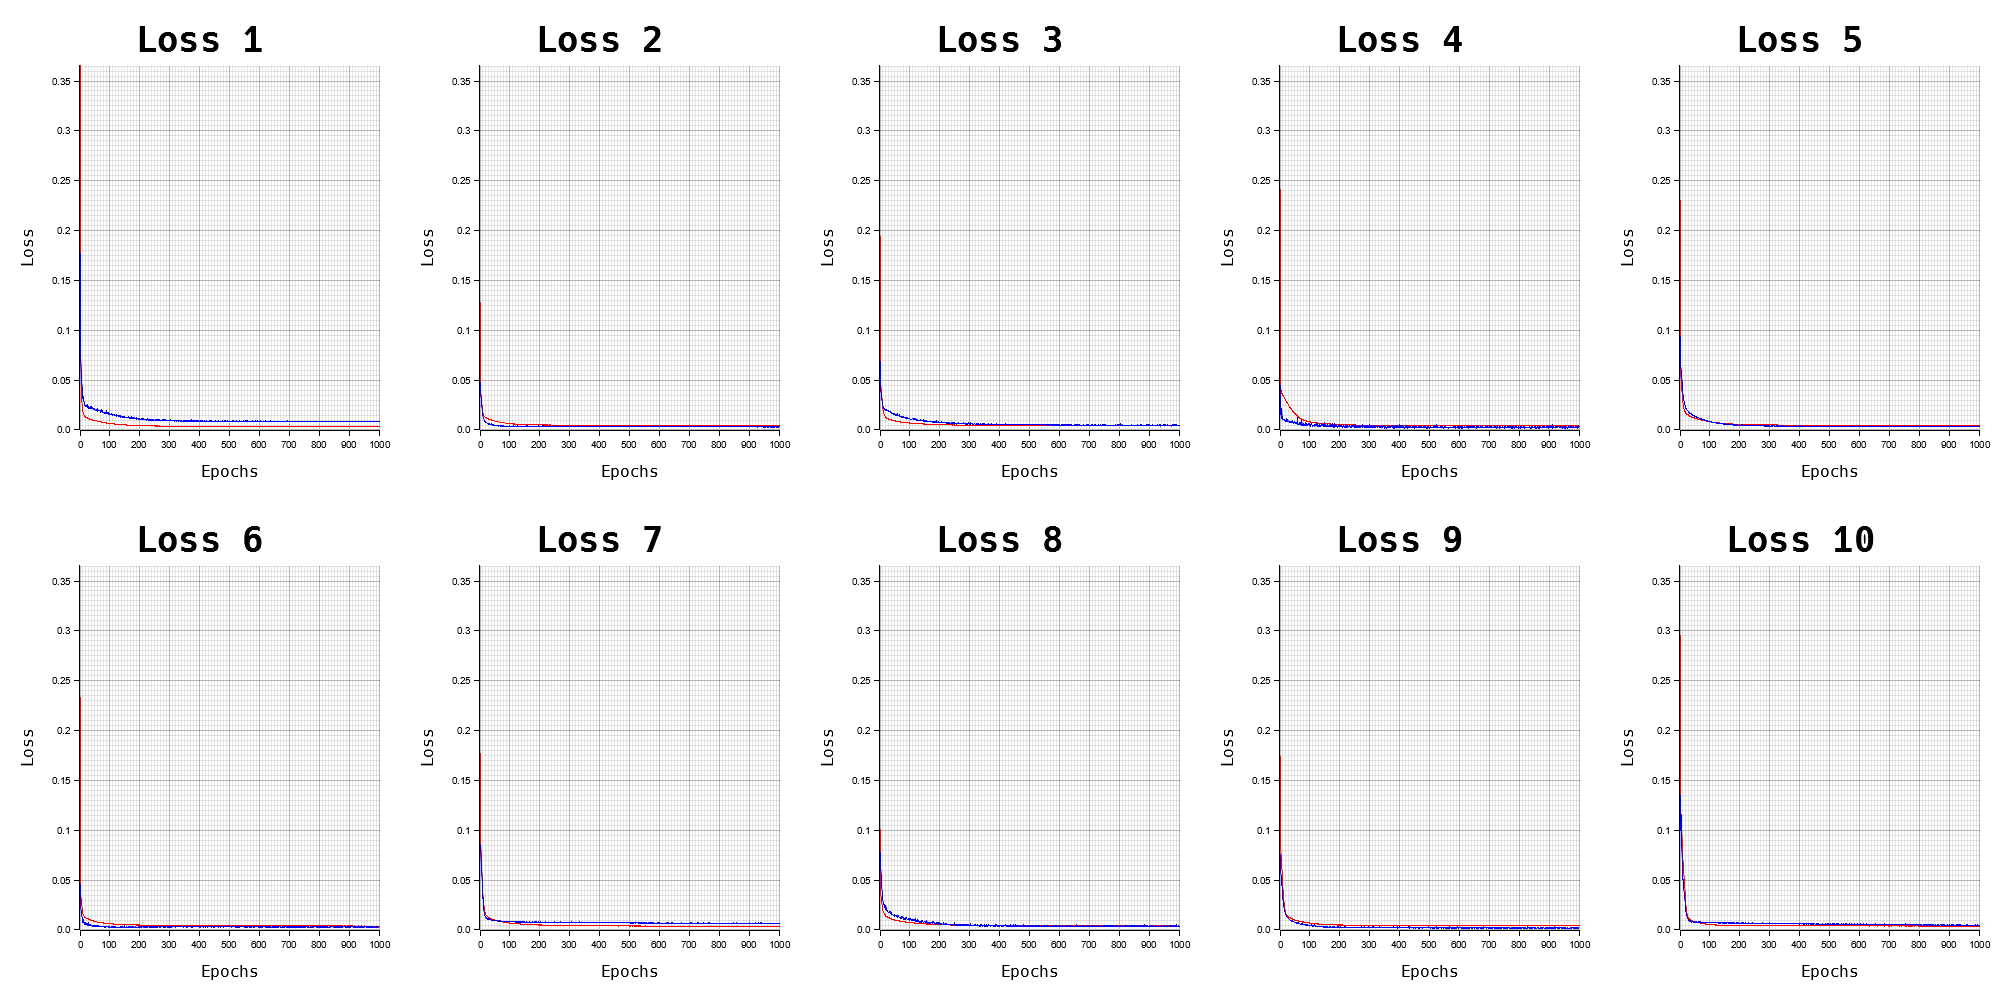
\includegraphics[width=\textwidth]{flood-8-4-1/loss}
		\caption{Each iteration training MSE (blue) and validation MSE (red) at each epoch.}
	\end{subfigure}
	\caption{Training result of Flood-8-4-1.}
	\label{fig:2}
\end{figure}
\FloatBarrier

\newpage
\subsubsection*{Flood-8-4-1 with no momentum}
Same base network but train with $lr = 0.01$ and $momentum = 0$.
\\ \\
Below is the graphs we get from training this network. The training process take about $60$ seconds.
\begin{figure}[ht]
	\begin{subfigure}{\textwidth}
		\centering
		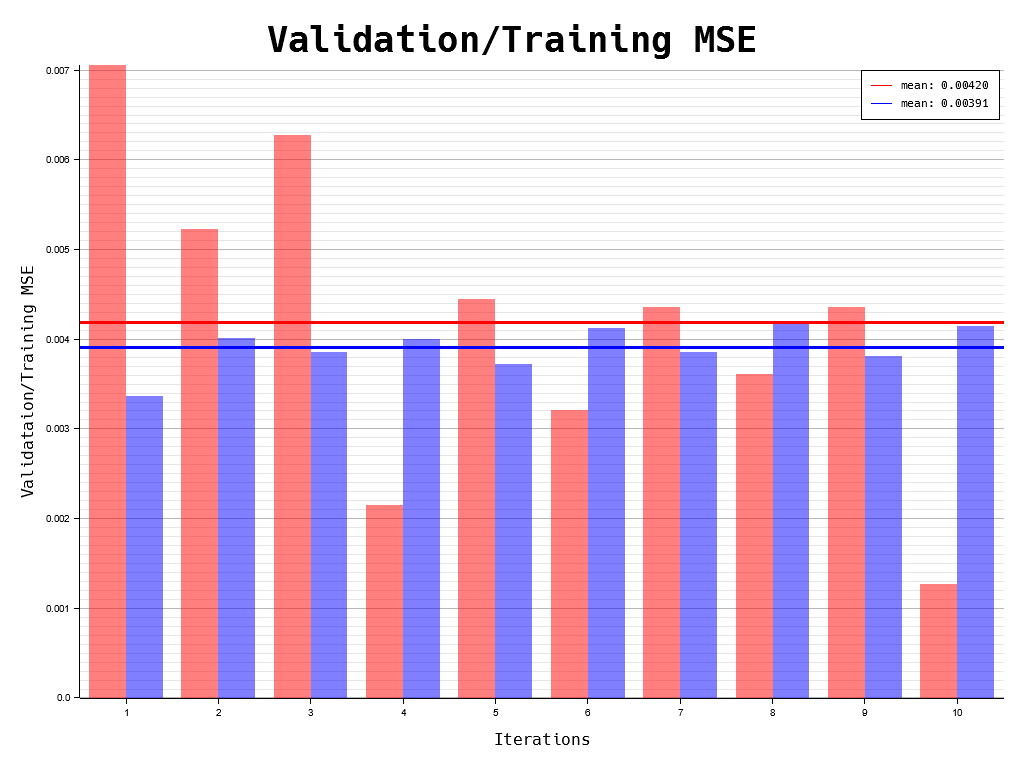
\includegraphics[scale=0.3]{flood-8-4-1_2/cv_l}
		\caption{Each iteration training (blue) and validation (red) MSE at last epoch}
	\end{subfigure}
	\begin{subfigure}{\textwidth}
		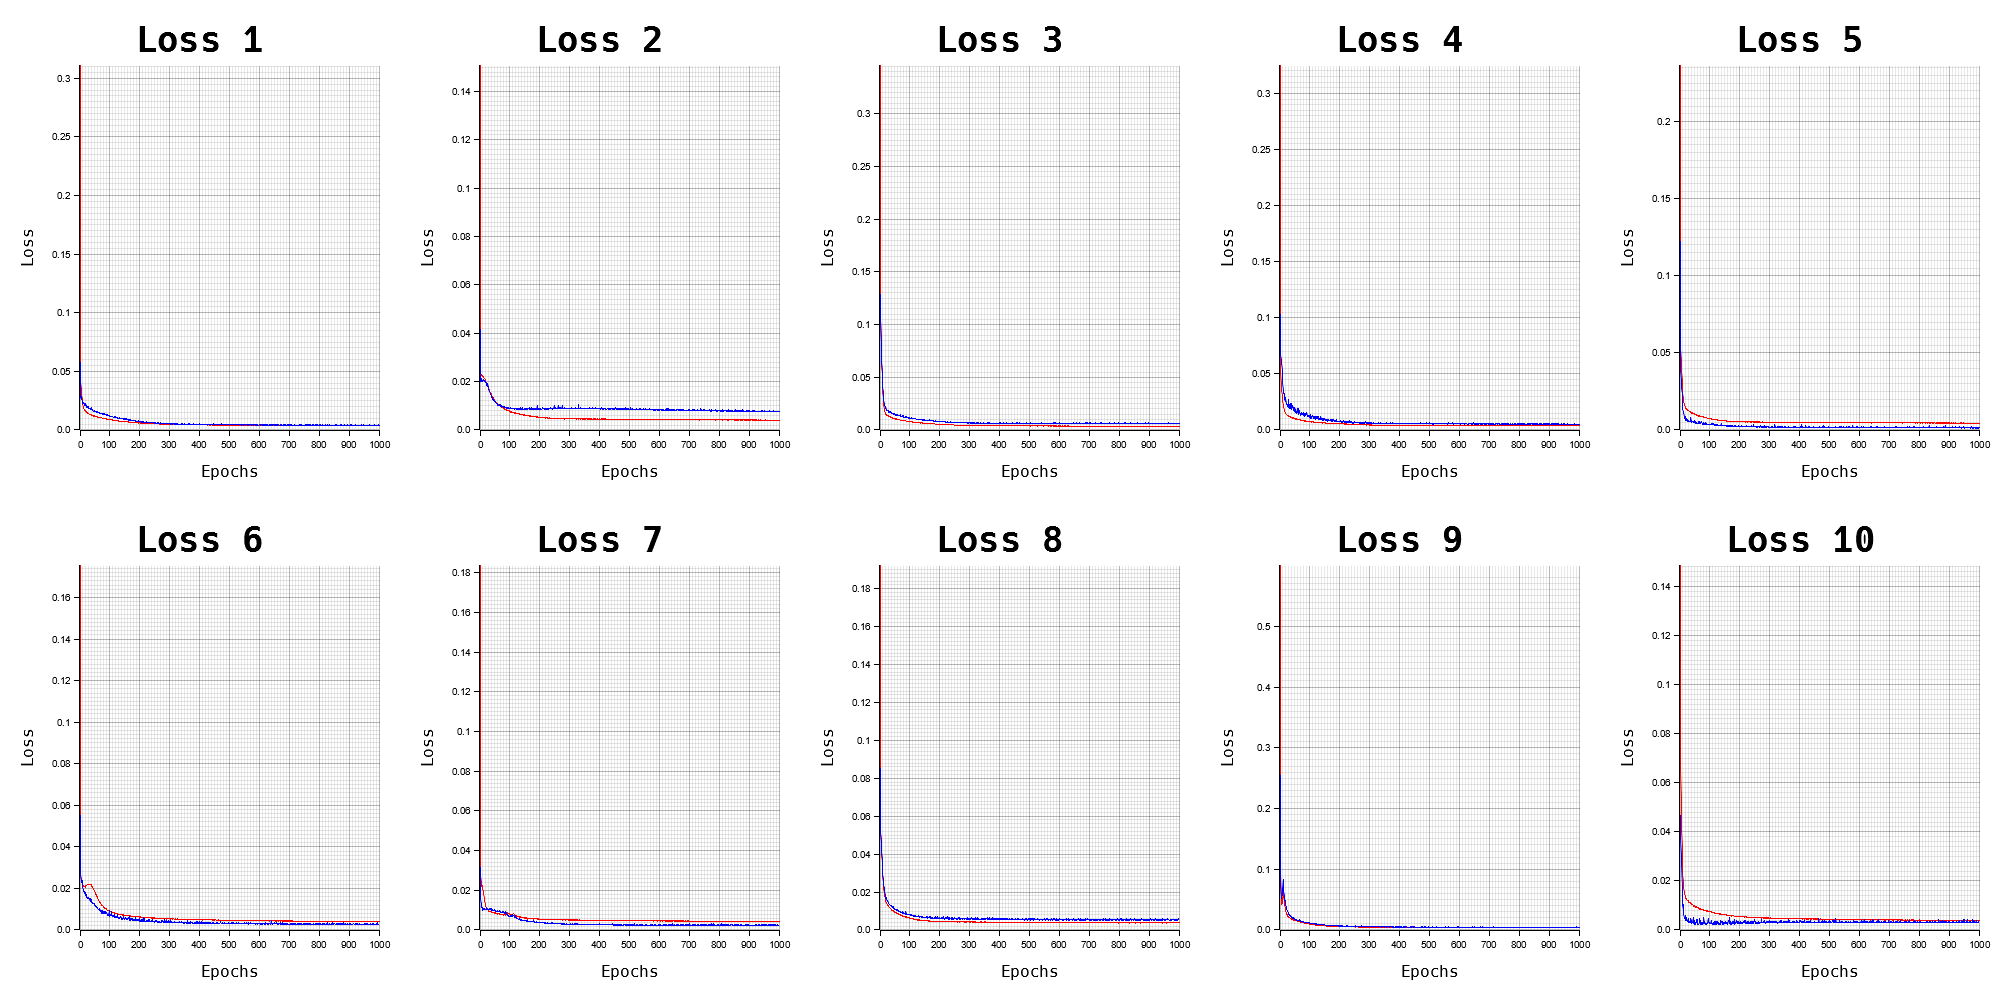
\includegraphics[width=\textwidth]{flood-8-4-1_2/loss}
		\caption{Each iteration training MSE (blue) and validation MSE (red) at each epoch.}
	\end{subfigure}
	\caption{Training result of Flood-8-4-1.}
	\label{fig:3}
\end{figure}
\FloatBarrier

\newpage
\subsubsection*{Flood-8-4-1 with small learning rate}
Same base network but train with $lr = 0.0001$ and $momentum = 0.01$.
\\ \\
Below is the graphs we get from training this network. The training process take about $59$ seconds.
\begin{figure}[ht]
	\begin{subfigure}{\textwidth}
		\centering
		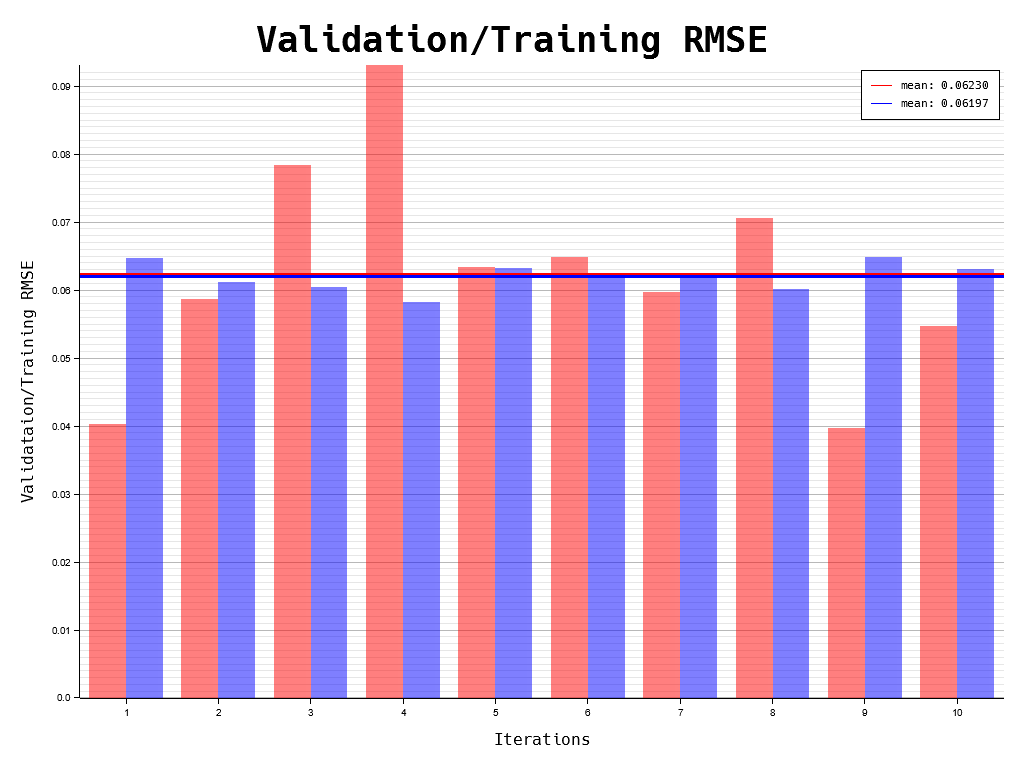
\includegraphics[scale=0.3]{flood-8-4-1_3/cv_l}
		\caption{Each iteration training (blue) and validation (red) MSE at last epoch}
	\end{subfigure}
	\begin{subfigure}{\textwidth}
		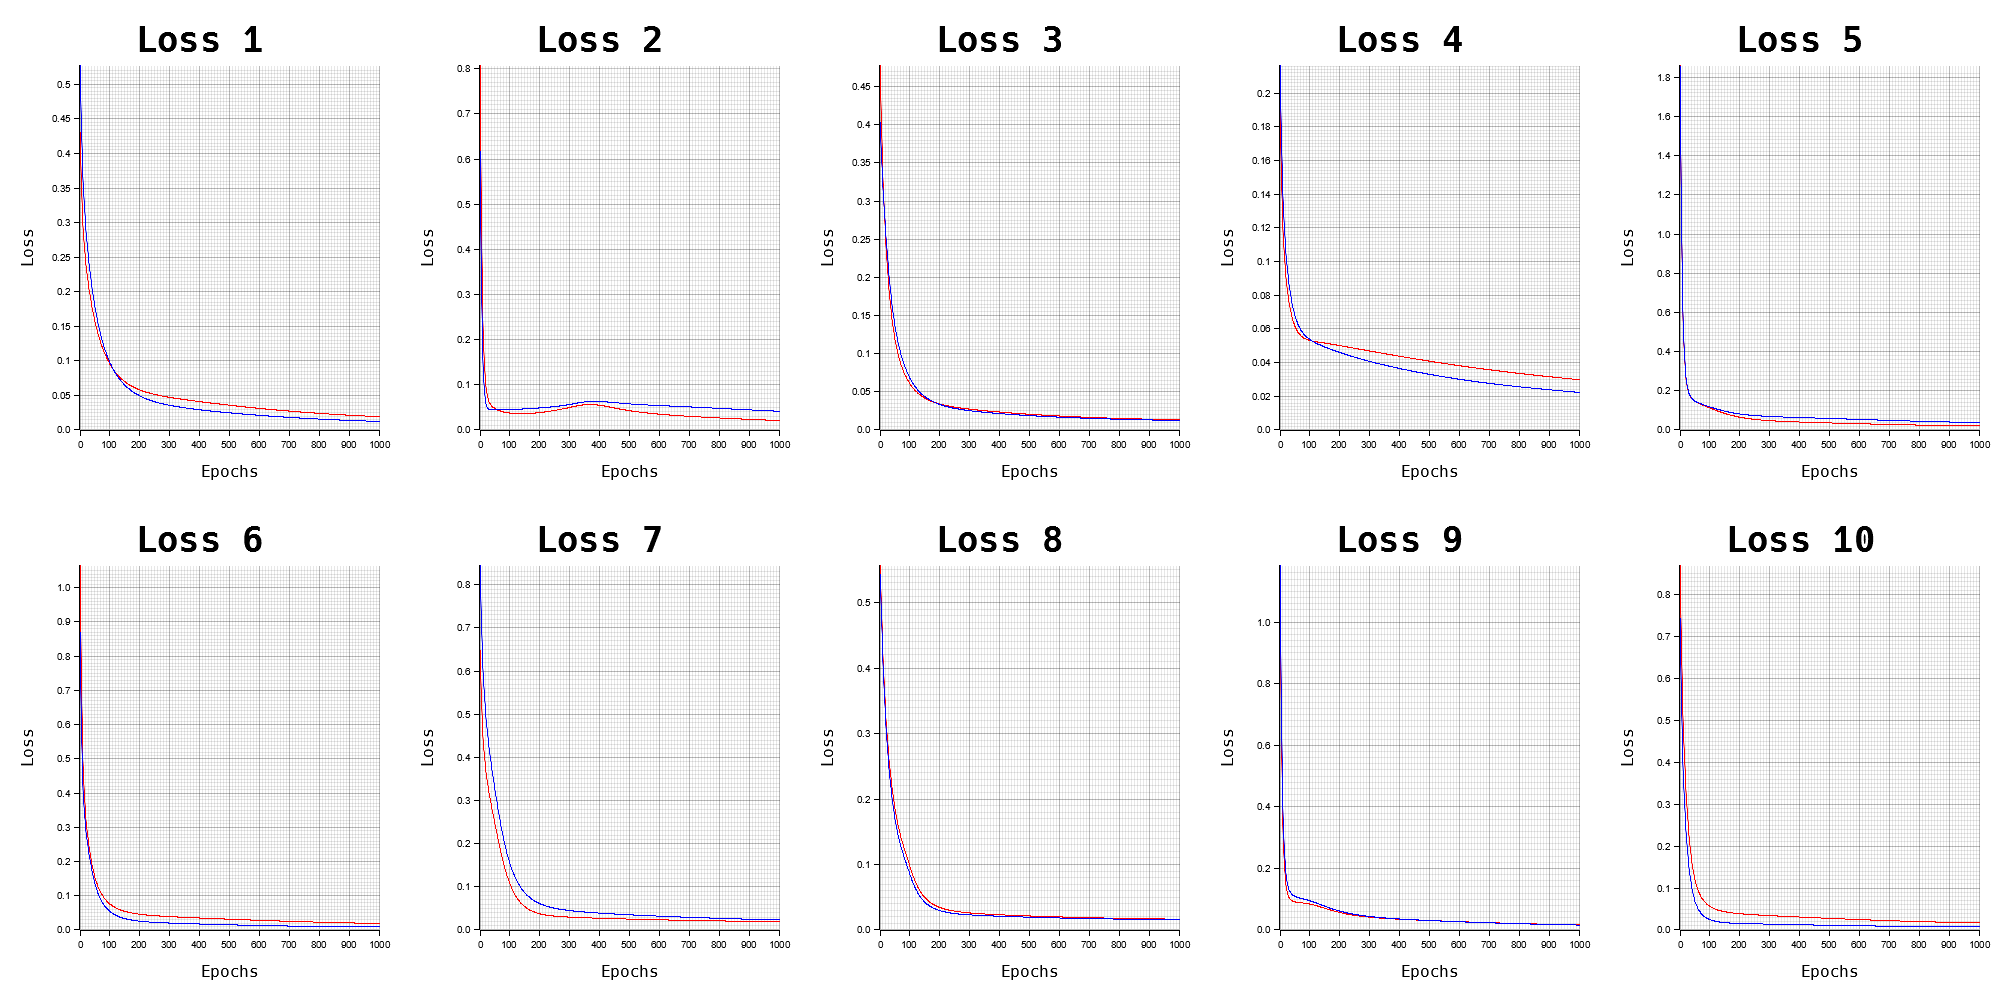
\includegraphics[width=\textwidth]{flood-8-4-1_3/loss}
		\caption{Each iteration training MSE (blue) and validation MSE (red) at each epoch.}
	\end{subfigure}
	\caption{Training result of Flood-8-4-1.}
	\label{fig:4}
\end{figure}
\FloatBarrier

\newpage
\subsubsection*{Flood-8-8-1}
Bigger network that contains 8 input nodes, 1 hidden layer with 8 nodes, and 1 output node train with $lr = 0.01$ and $momentum = 0.01$.
\\ \\
Below is the graphs we get from training this network. The training process take about $105$ seconds.
\begin{figure}[ht]
	\begin{subfigure}{\textwidth}
		\centering
		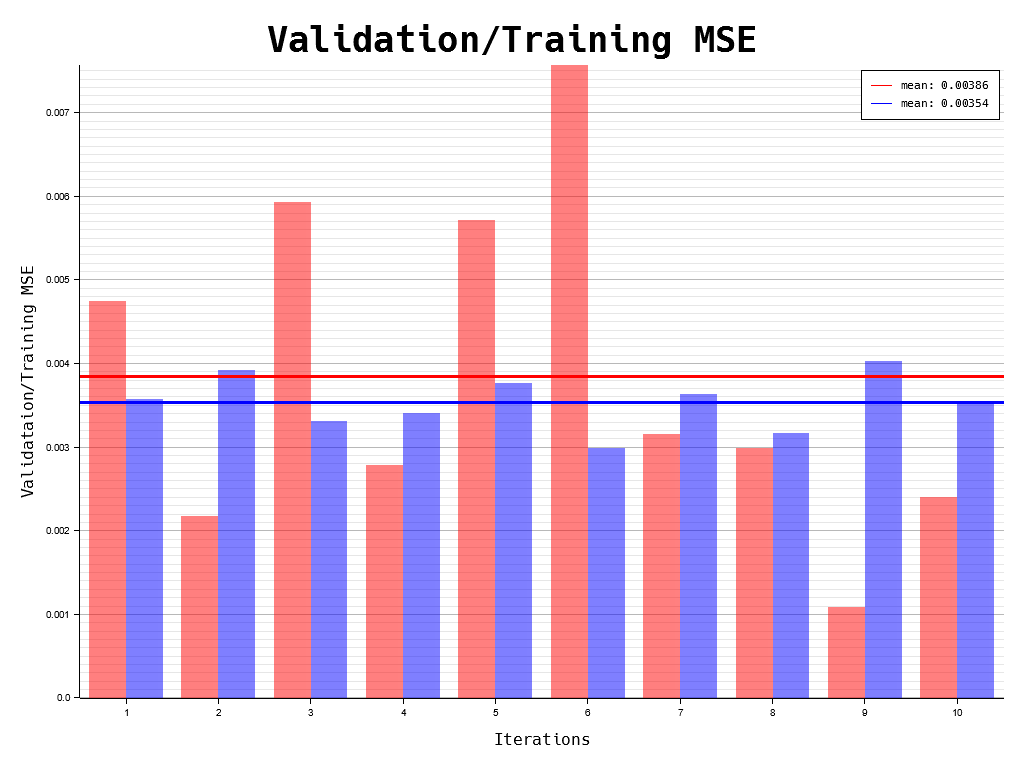
\includegraphics[scale=0.3]{flood-8-8-1/cv_l}
		\caption{Each iteration training (blue) and validation (red) MSE at last epoch}
	\end{subfigure}
	\begin{subfigure}{\textwidth}
		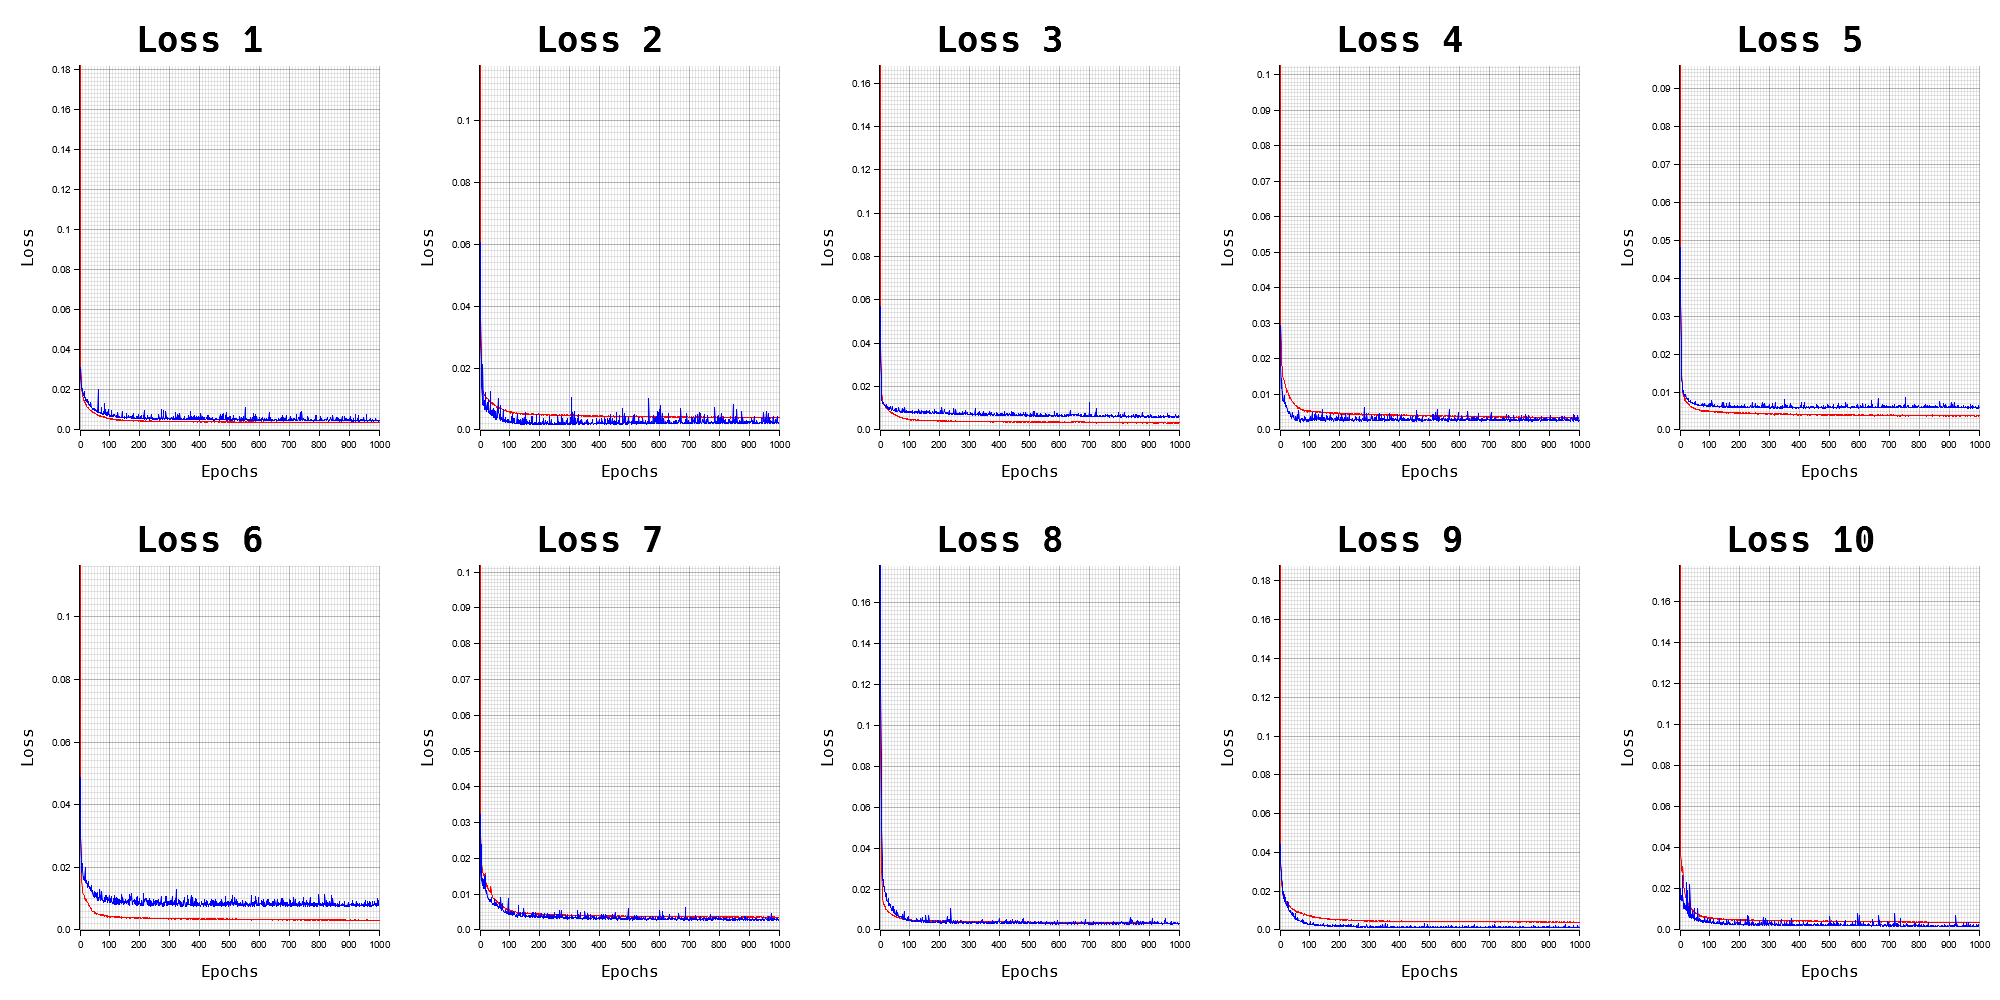
\includegraphics[width=\textwidth]{flood-8-8-1/loss}
		\caption{Each iteration training MSE (blue) and validation MSE (red) at each epoch.}
	\end{subfigure}
	\caption{Training result of Flood-8-4-1.}
	\label{fig:5}
\end{figure}
\FloatBarrier

\newpage
\subsection*{Analysis}
From \cref{table:1}, we can see that network with same size will use around the same amount of training time, but with bigger network the training time get longer. We can also see that Flood-8-4-1 with small learning rate is not performing well (has the biggest validation set mean MSE) compare with other network, the network seem to be stuck at this gradient level (see \cref{fig:4} the network is slowly converging but too slow). Lastly, we can also see that the best performing network Flood-8-8-1's validation set mean MSE is not much better than Flood-8-4-1 and Flood-8-4-1 with no momentum, the biggest different is just $0.34 \times 10^{-3}$.

\begin{table}[htp]
	\centering
	\begin{tabular}{l S[table-format=3] S[table-format=2.2]}
		\toprule
        \multicolumn{1}{c}{Model} & {Training Time (seconds)} & {Validation Set Mean MSE ($10^{-3}$)} \\
        \midrule
        Flood-8-4-1 & 60 & 4.03 \\
        Flood-8-4-1 with no momentum & 60 & 4.20 \\
        Flood-8-4-1 with small learniing rate & 59 & 19.83 \\
        Flood-8-8-1 & 105 & 3.86 \\
        \bottomrule
    \end{tabular}
    \caption{Training time and validation mean MSE (blue line on (a) \cref{fig:2} - \cref{fig:5} ) of each Flood network.}
	\label{table:1}
\end{table}
\FloatBarrier

\newpage
\section{CrossPat Dataset}
\subsection*{Problem}
We want to predict the class (1 of possible 2 classes) that belong to our inputs (or features).

\begin{figure}[ht]
	\centering
	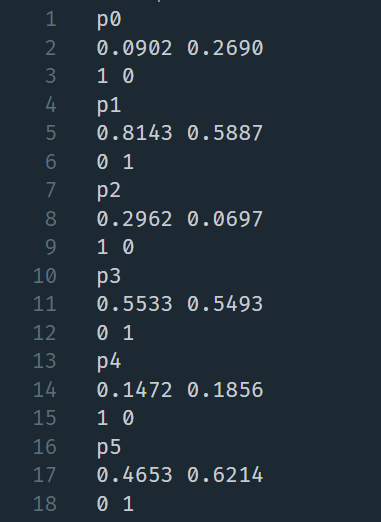
\includegraphics[scale=0.5]{cross_data}
	\caption{Examples of given data where p$x$ is an object and first line after it is its features, second line is its class}
\end{figure}
\FloatBarrier

\subsection*{Parameters Setting}
\begin{itemize}
	\item All nodes use $sigmoid$ as an activation function.
	\item Weights is a random number between $[-1, 1]$
	\item Each layer's bias is $1$
	\item Use MSE (Mean Squared Error) as a loss function.
\end{itemize}

\subsection*{Training}
Use 10\% cross-validation with no data preprocessing, and train with SGD (Stochastic Gradient Descent) algorithm. Then, we train each cross-validation set for $5000$ epochs.
\\ \\
We will create one base network that should perform good enough and create a variation base on that network, that is train with no \emph{momentum}, train with smaller \emph{learning rate}, and add more layers or hidden nodes to see that if we introduce those variations, will the network perform better, converge faster or no improvement at all?

\subsection*{Training Result}
Accuracy is calculate using this equation $\frac{TP+TN}{TP+TN+FN+FP}$ where $TP, TN, FN, FP$ comes from confustion matrix.
\subsubsection*{Cross-2-4-1}
Our base network with 2 input nodes, 1 hidden layer with 4 nodes, and 1 output node train with $lr = 0.01$ and $momentum = 0.01$. We use only 1 output node because this is a binary classification task so we can just map a pair $(1, 0) \rightarrow 1$ and $(0, 1) \rightarrow 0$
\subsubsection*{Cross-2-4-1 with no momentum}
Same base network train with $lr = 0.01$ and $momentum = 0.0$.
\subsubsection*{Cross-2-4-1 with smaller learning rate}
Same base network train with $lr = 0.0001$ and $momentum = 0.01$.
\subsubsection*{Cross-2-8-1}
Bigger network that contains 2 input nodes, 1 hidden layer with 4 nodes, and 1 output node train with $lr = 0.01$ and $momentum = 0.01$.

\begin{figure}[ht]
	\begin{subfigure}{\textwidth}
		\centering
		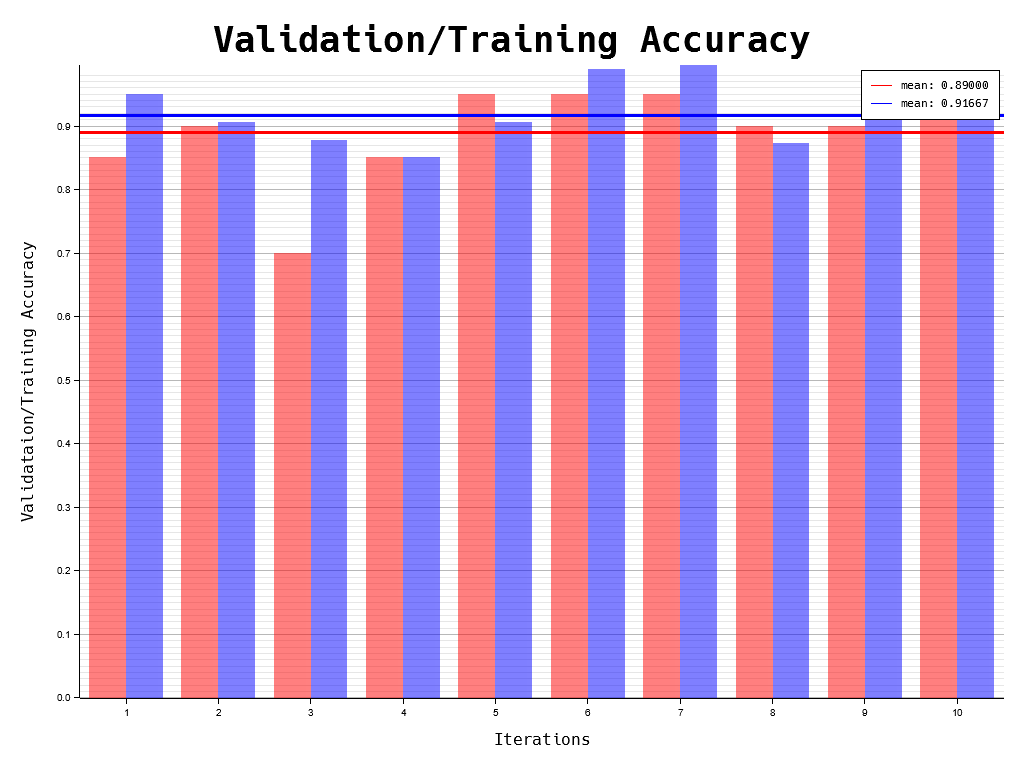
\includegraphics[width=0.5\textwidth]{cross-2-4-1/acc}
		\caption{Each iteration training (blue) and validation (red) set accuracy at last epoch}
	\end{subfigure}
	\begin{subfigure}{\textwidth}
		\centering
		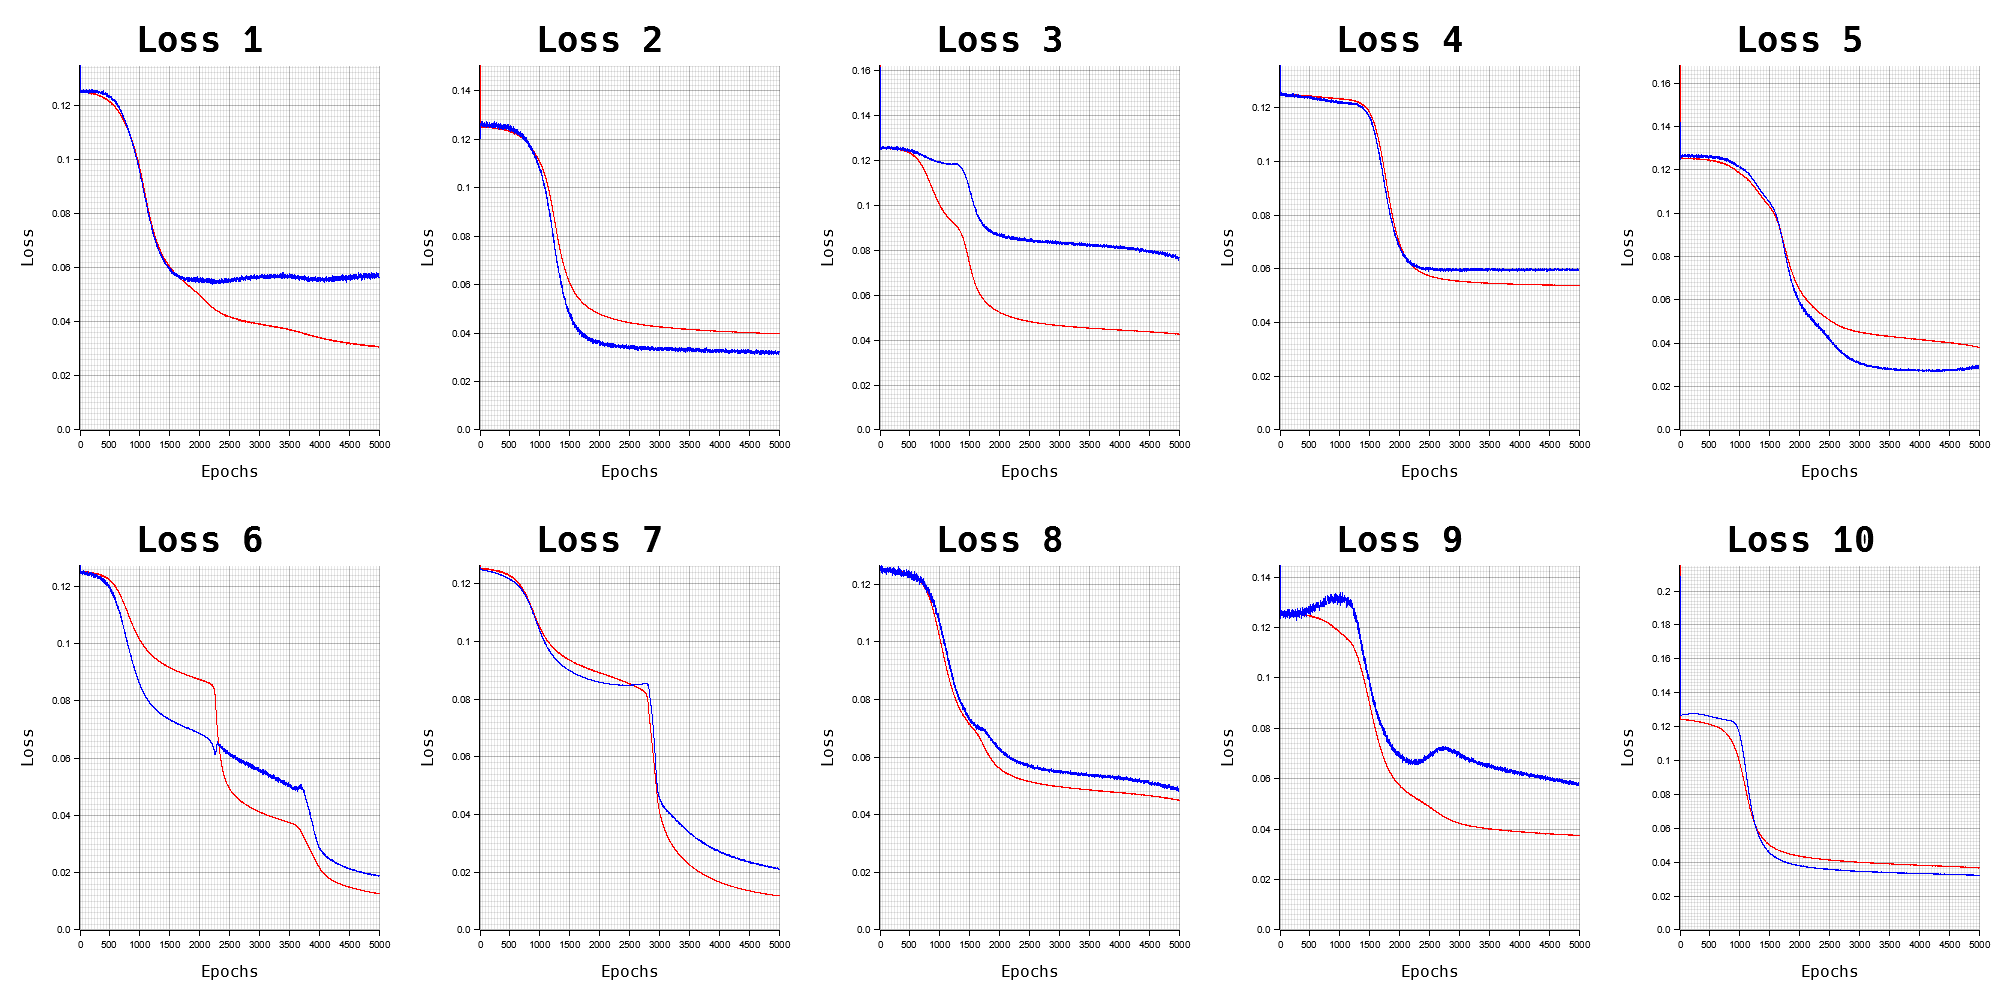
\includegraphics[width=0.9\textwidth]{cross-2-4-1/loss}
		\caption{Each iteration training MSE (blue) and validation MSE (red) at each epoch.}
	\end{subfigure}
	\begin{subfigure}{\textwidth}
		\centering
		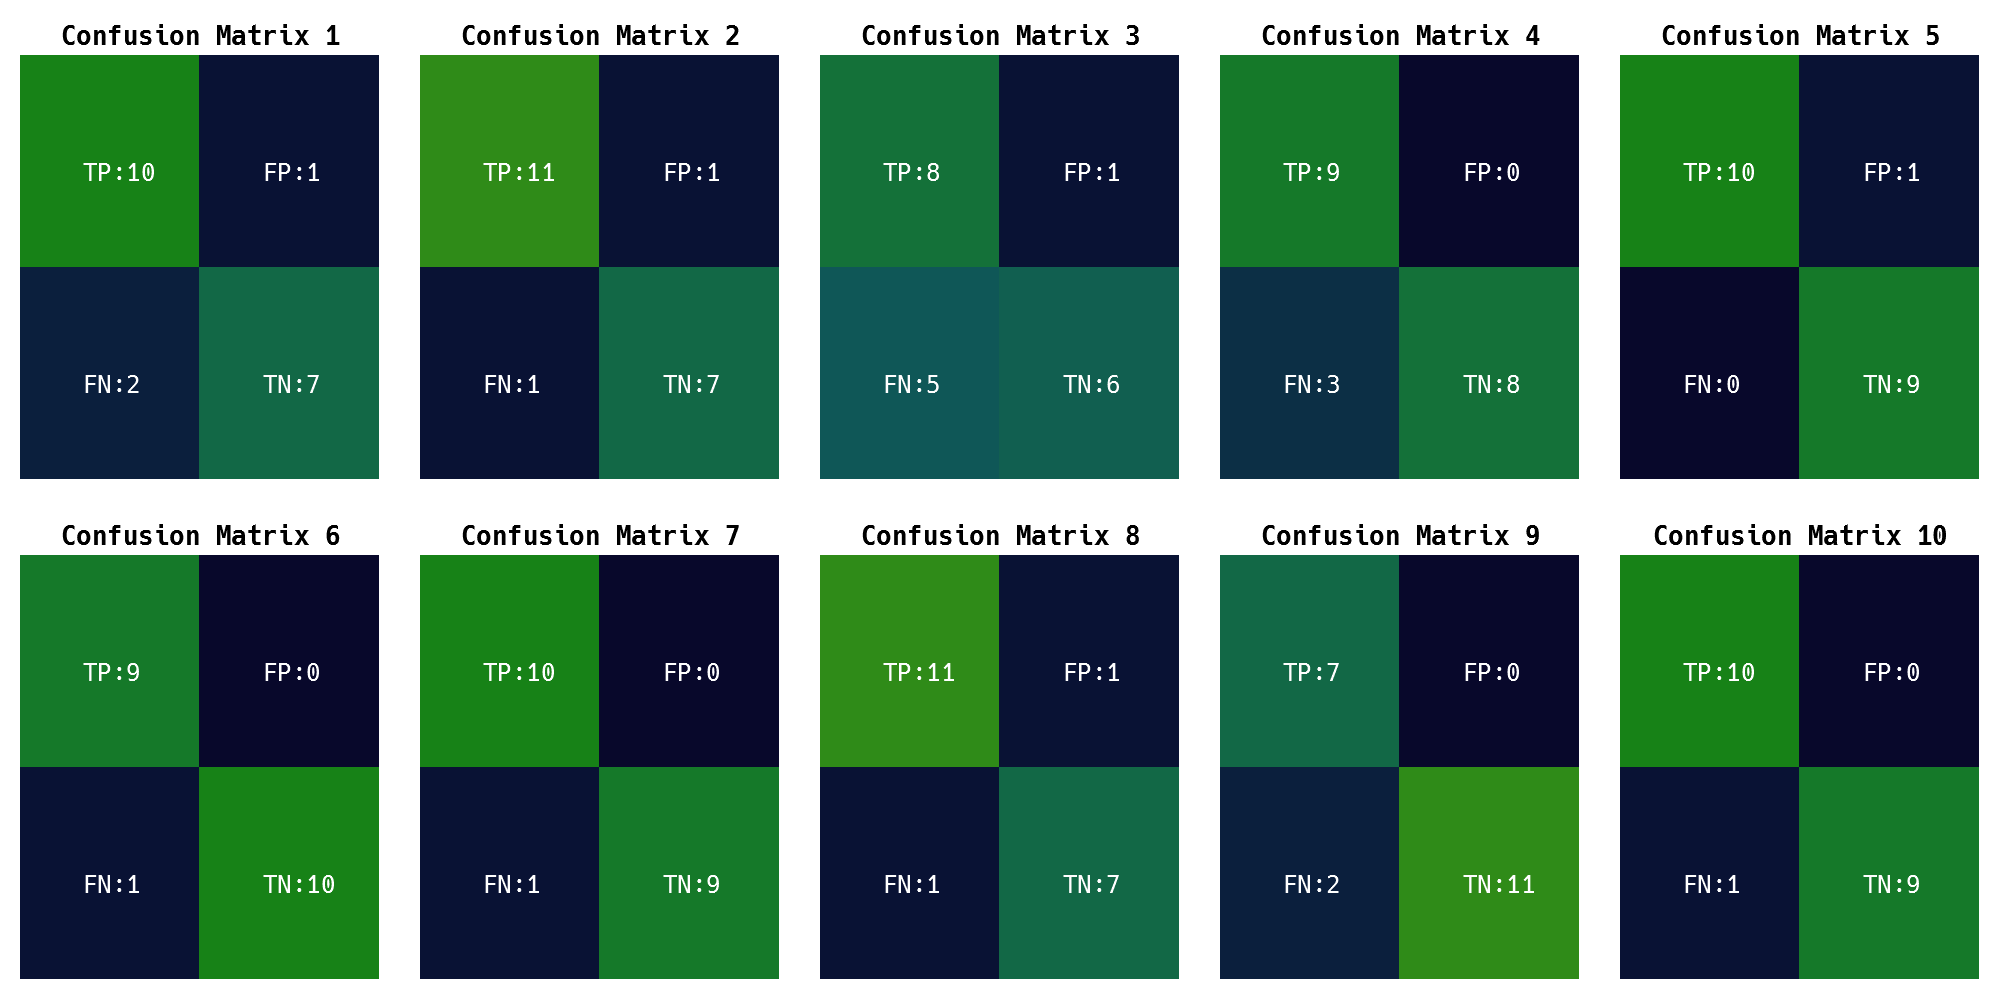
\includegraphics[width=0.9\textwidth]{cross-2-4-1/confusion_matrix}
		\caption{Each iterations validation set confusion matrix where y-axis is an actual class $1, 0$ top to bottom and x-axis is predicted class $1, 0$ left to right.}
	\end{subfigure}
	\caption{Training result of Cross-2-4-1.}
	\label{fig:7}
\end{figure}
\FloatBarrier

\begin{figure}[ht]
	\begin{subfigure}{\textwidth}
		\centering
		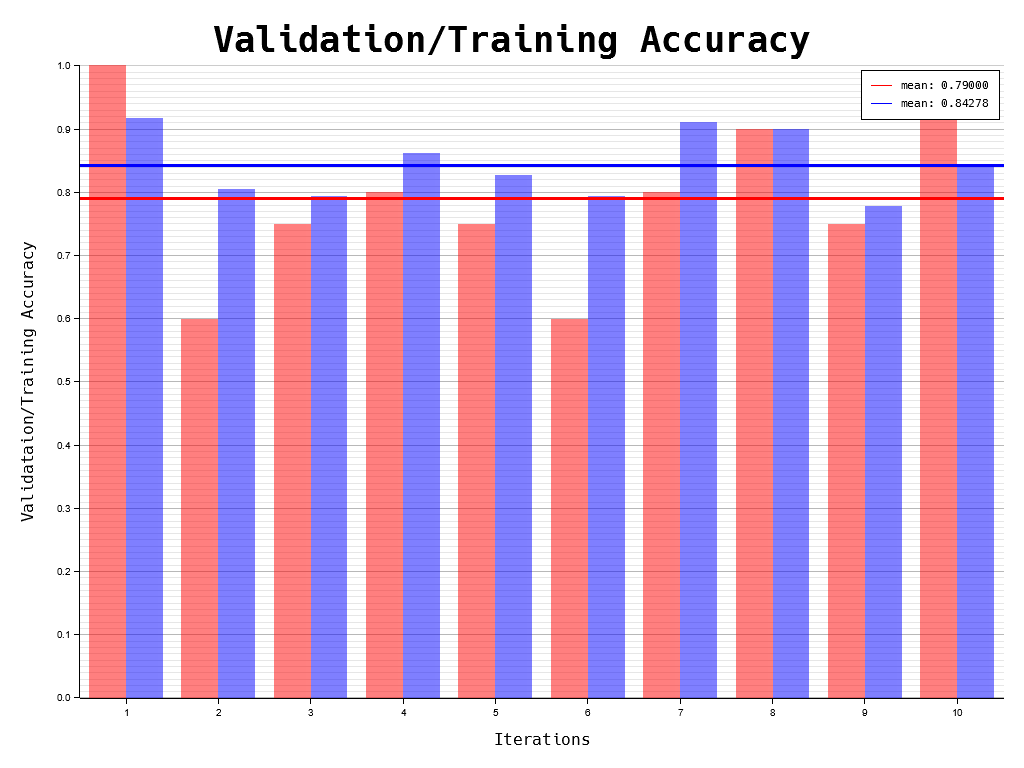
\includegraphics[width=0.5\textwidth]{cross-2-4-1_2/acc}
		\caption{Each iteration training (blue) and validation (red) set accuracy at last epoch}
	\end{subfigure}
	\begin{subfigure}{\textwidth}
		\centering
		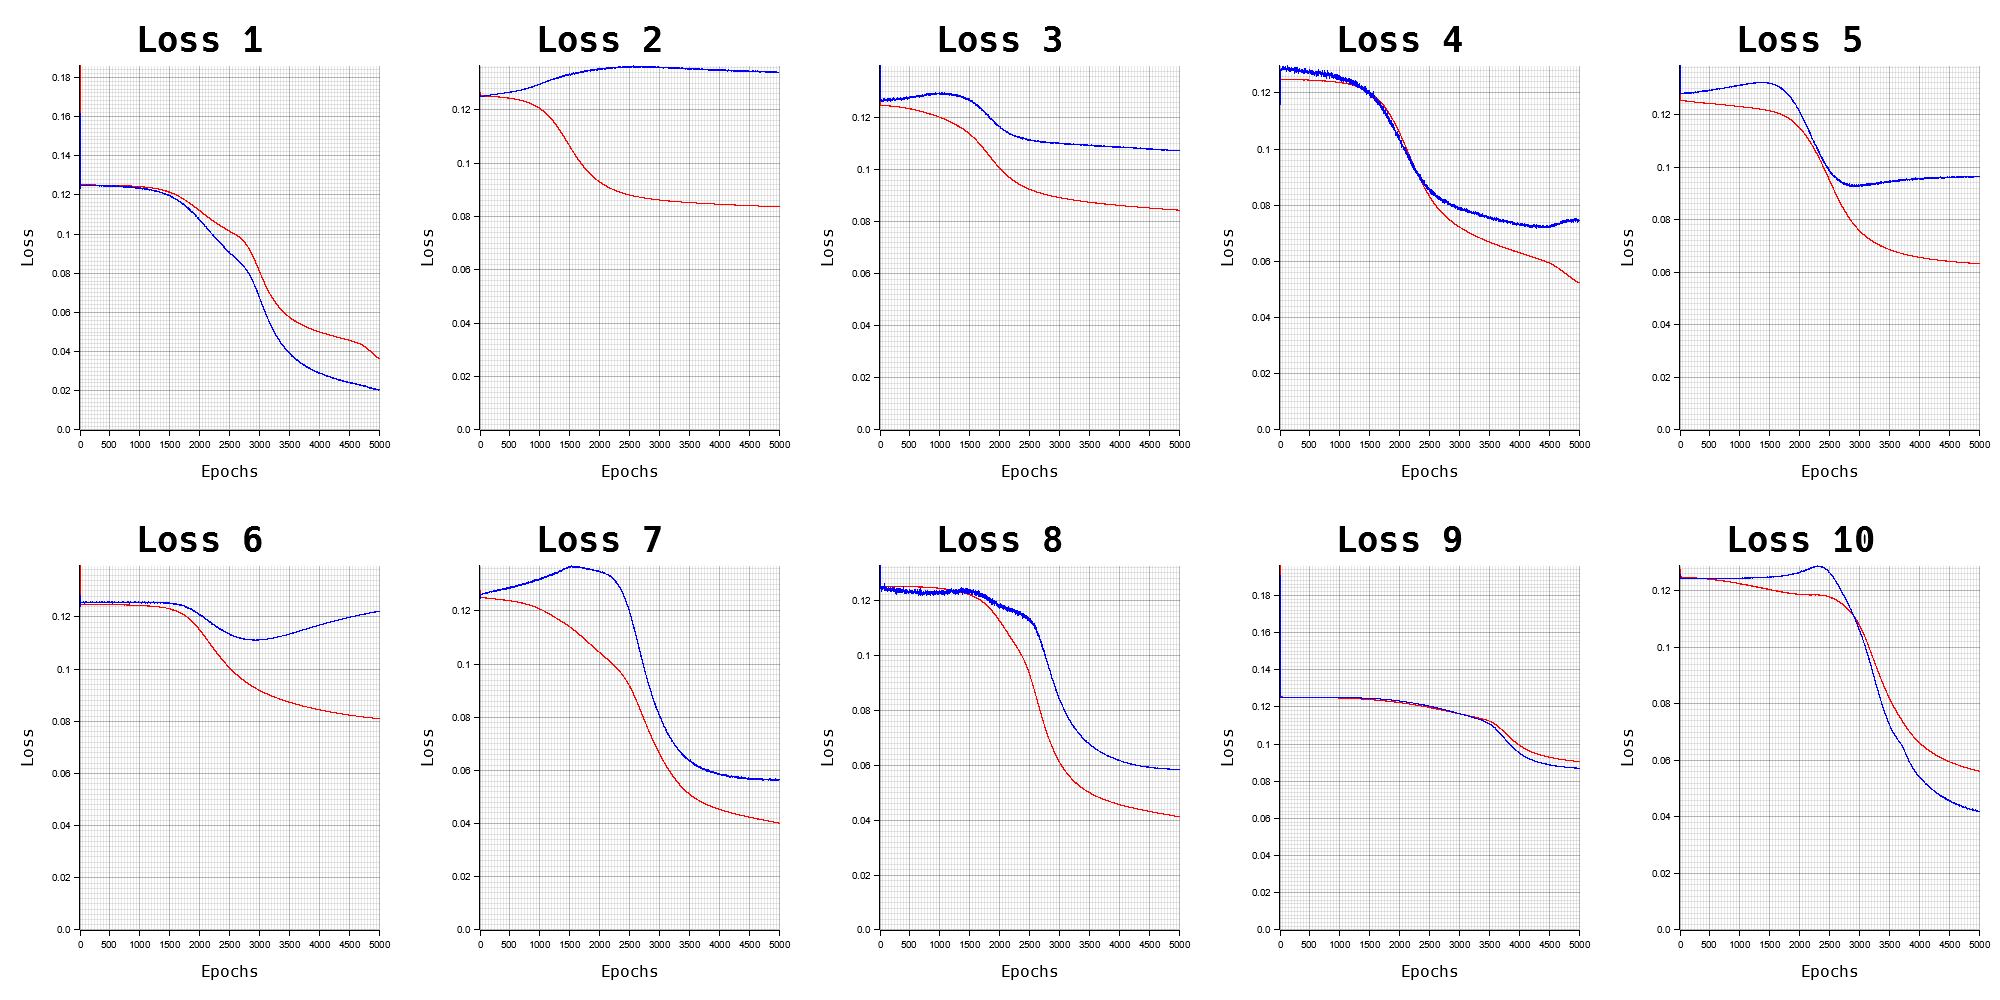
\includegraphics[width=0.9\textwidth]{cross-2-4-1_2/loss}
		\caption{Each iteration training MSE (blue) and validation MSE (red) at each epoch.}
	\end{subfigure}
	\begin{subfigure}{\textwidth}
		\centering
		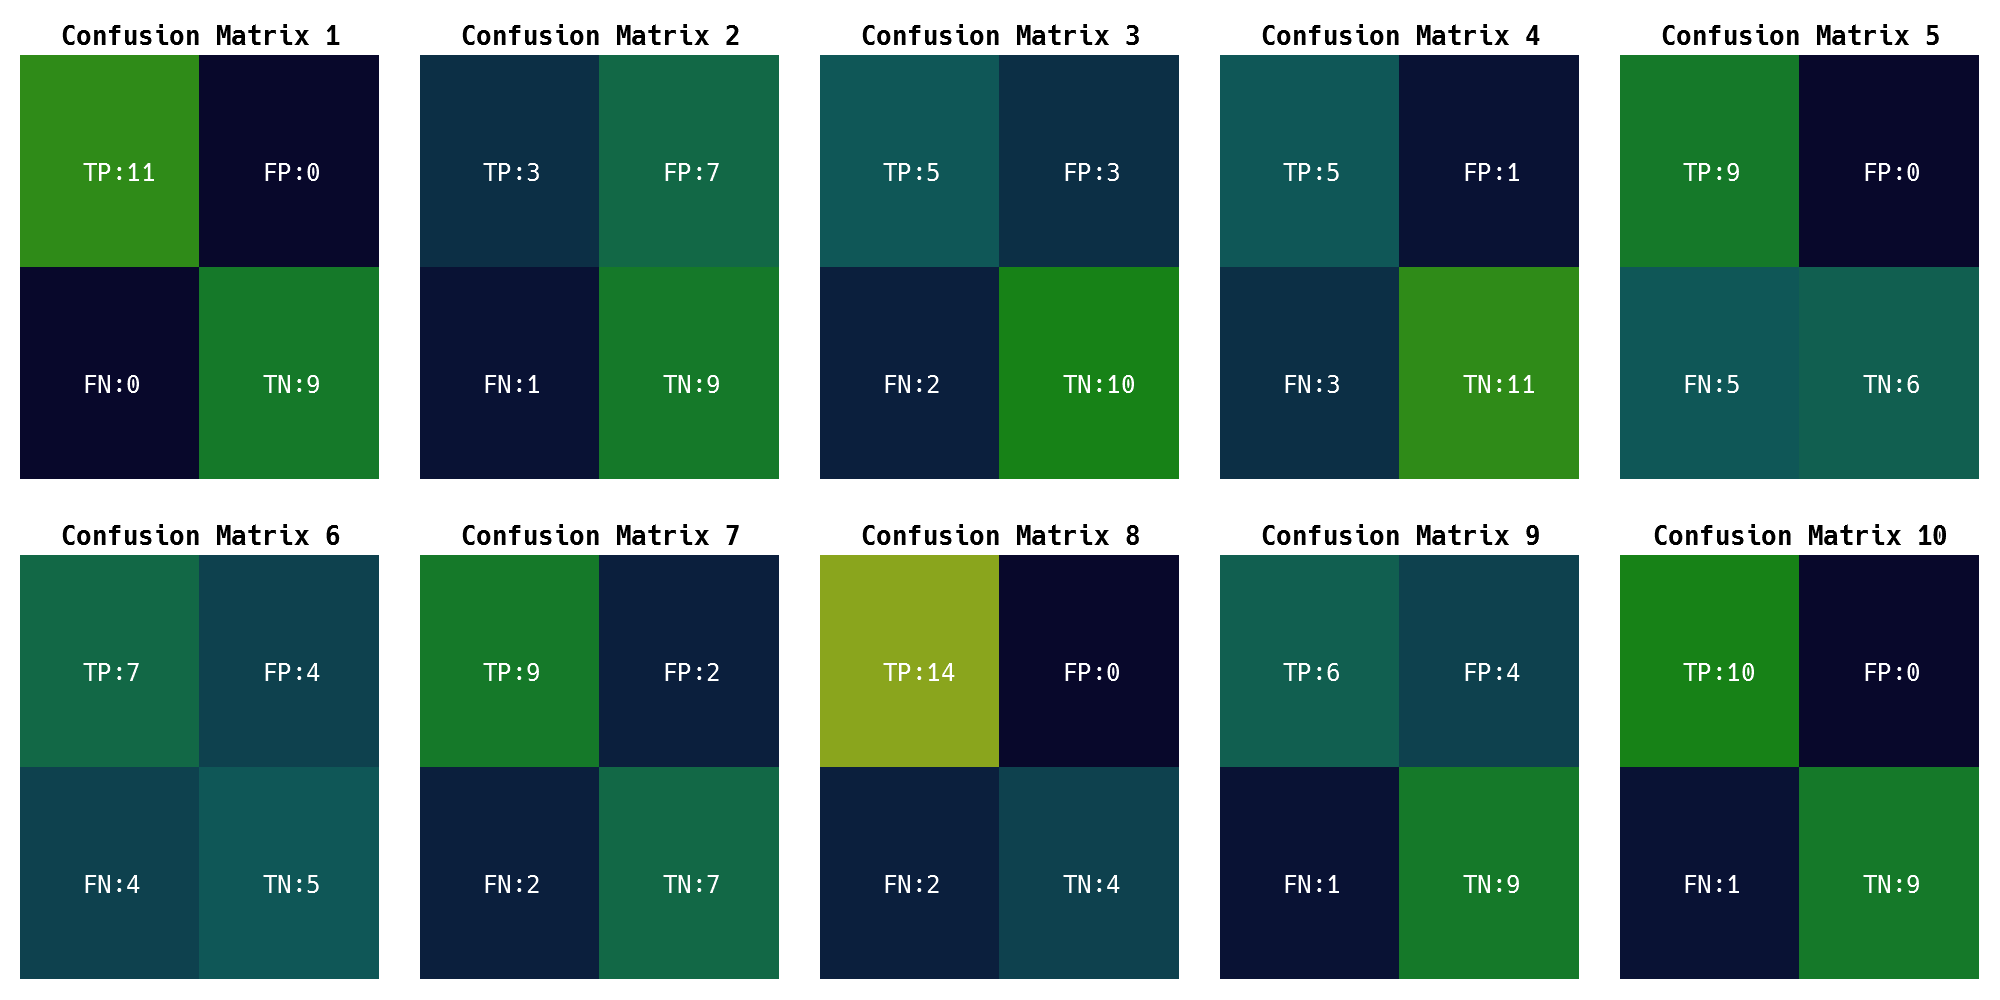
\includegraphics[width=0.9\textwidth]{cross-2-4-1_2/confusion_matrix}
		\caption{Each iterations validation set confusion matrix where y-axis is an actual class $1, 0$ top to bottom and x-axis is predicted class $1, 0$ left to right.}
	\end{subfigure}
	\caption{Training result of Cross-2-4-1.}
	\label{fig:8}
\end{figure}
\FloatBarrier

\begin{figure}[ht]
	\begin{subfigure}{\textwidth}
		\centering
		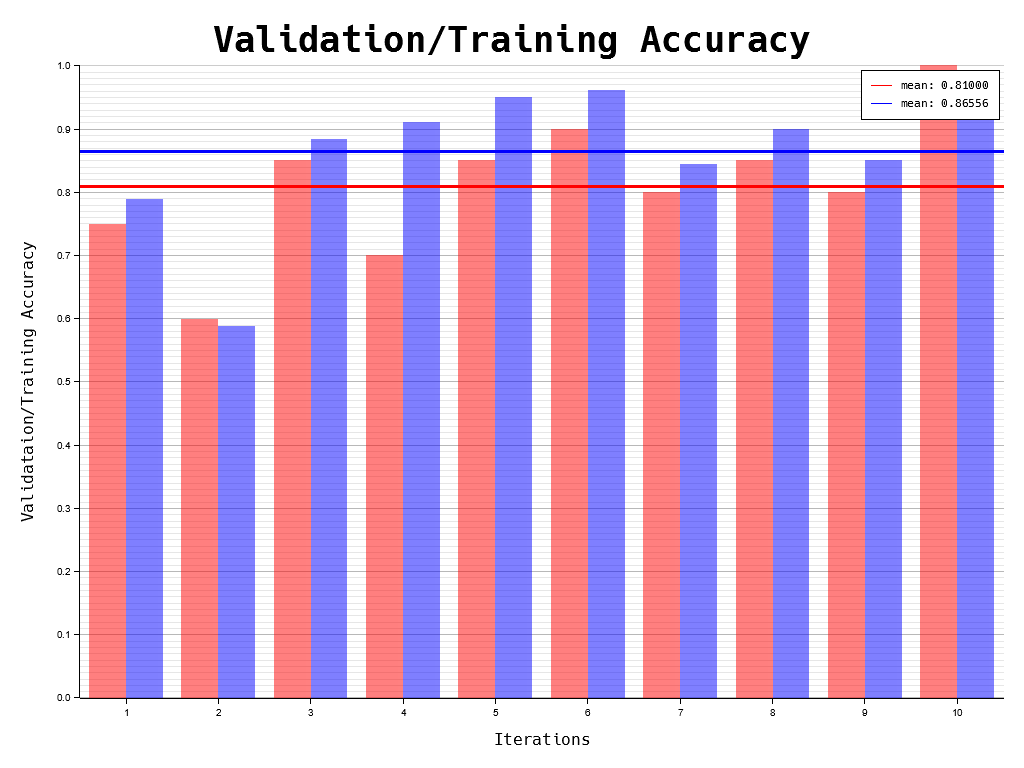
\includegraphics[width=0.5\textwidth]{cross-2-4-1_3/acc}
		\caption{Each iteration training (blue) and validation (red) set accuracy at last epoch}
	\end{subfigure}
	\begin{subfigure}{\textwidth}
		\centering
		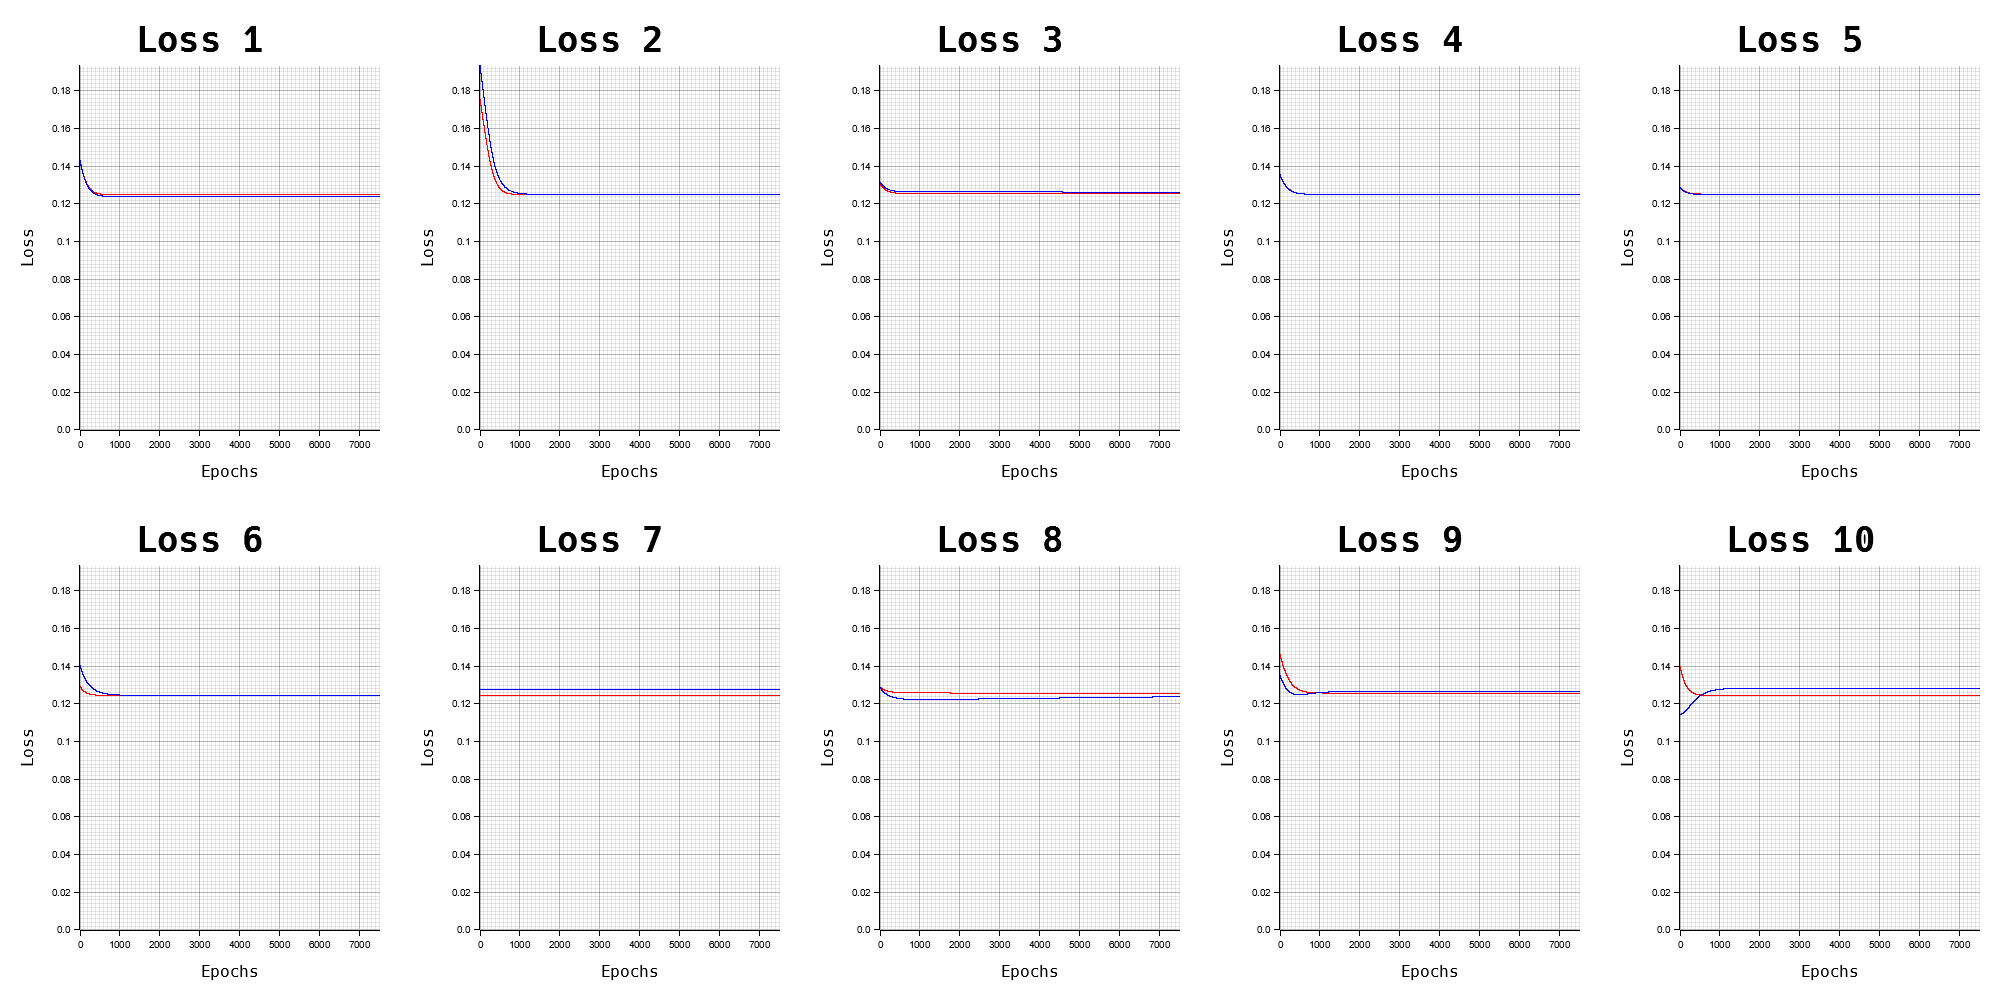
\includegraphics[width=0.9\textwidth]{cross-2-4-1_3/loss}
		\caption{Each iteration training MSE (blue) and validation MSE (red) at each epoch.}
	\end{subfigure}
	\begin{subfigure}{\textwidth}
		\centering
		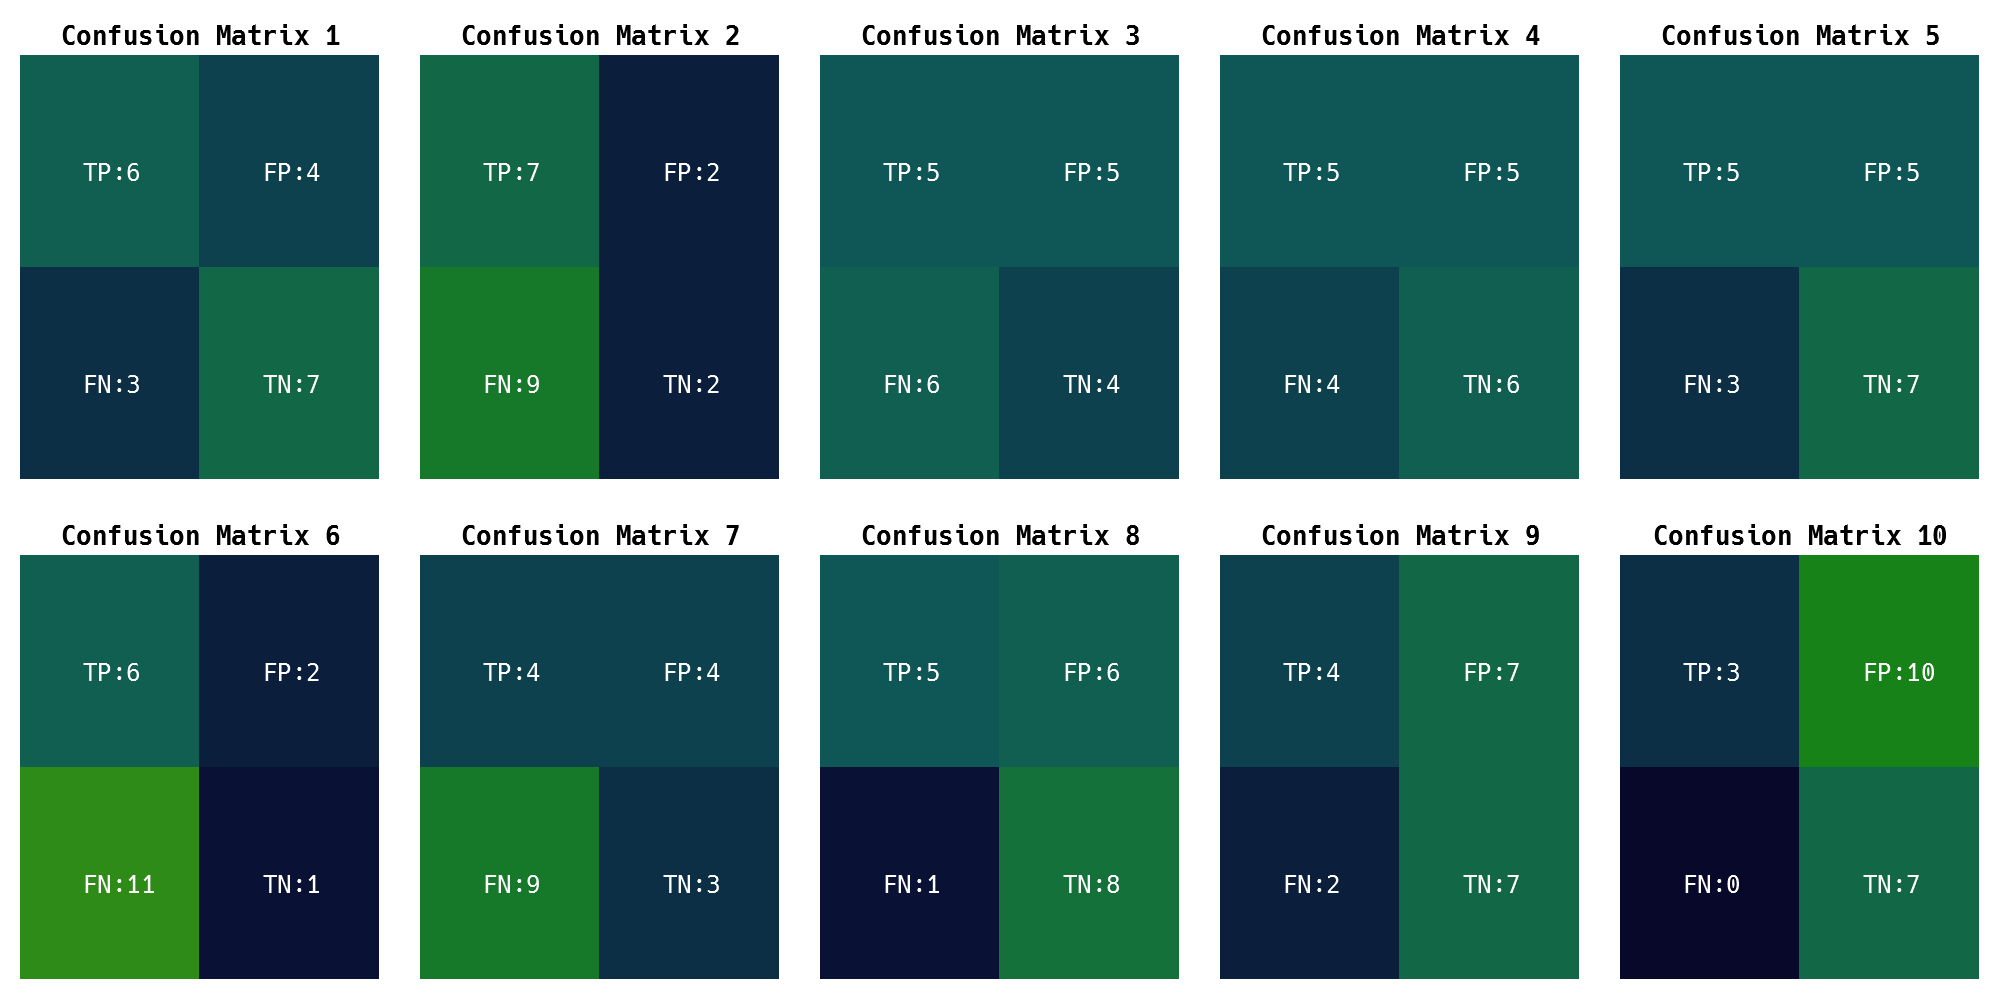
\includegraphics[width=0.9\textwidth]{cross-2-4-1_3/confusion_matrix}
		\caption{Each iterations validation set confusion matrix where y-axis is an actual class $1, 0$ top to bottom and x-axis is predicted class $1, 0$ left to right.}
	\end{subfigure}
	\caption{Training result of Cross-2-4-1.}
	\label{fig:9}
\end{figure}
\FloatBarrier

\begin{figure}[ht]
	\begin{subfigure}{\textwidth}
		\centering
		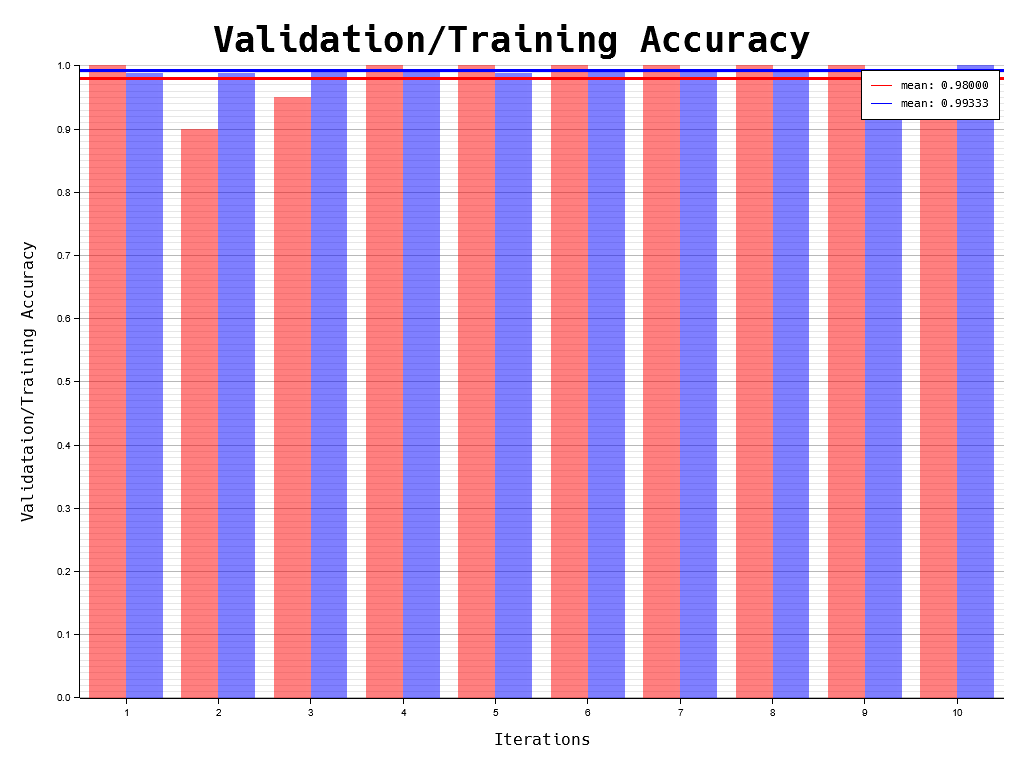
\includegraphics[width=0.5\textwidth]{cross-2-8-1/acc}
		\caption{Each iteration training (blue) and validation (red) set accuracy at last epoch}
	\end{subfigure}
	\begin{subfigure}{\textwidth}
		\centering
		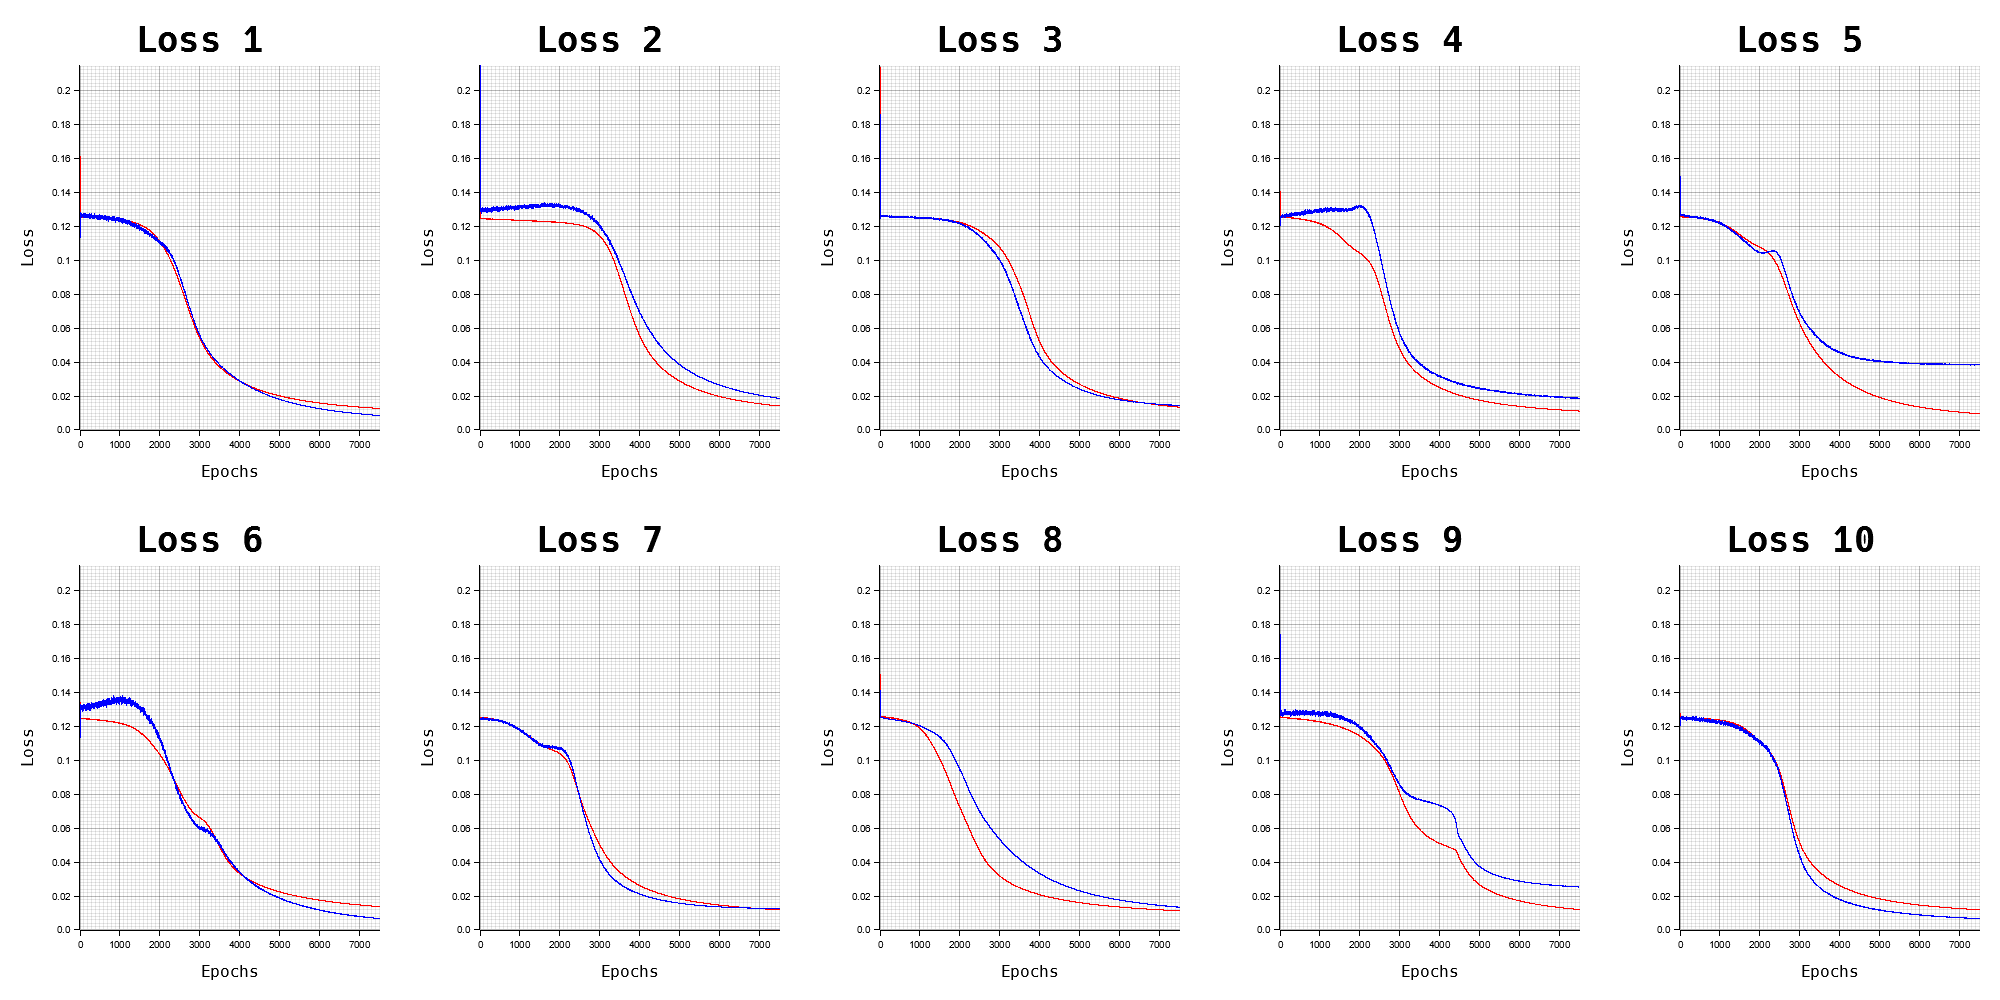
\includegraphics[width=0.9\textwidth]{cross-2-8-1/loss}
		\caption{Each iteration training MSE (blue) and validation MSE (red) at each epoch.}
	\end{subfigure}
	\begin{subfigure}{\textwidth}
		\centering
		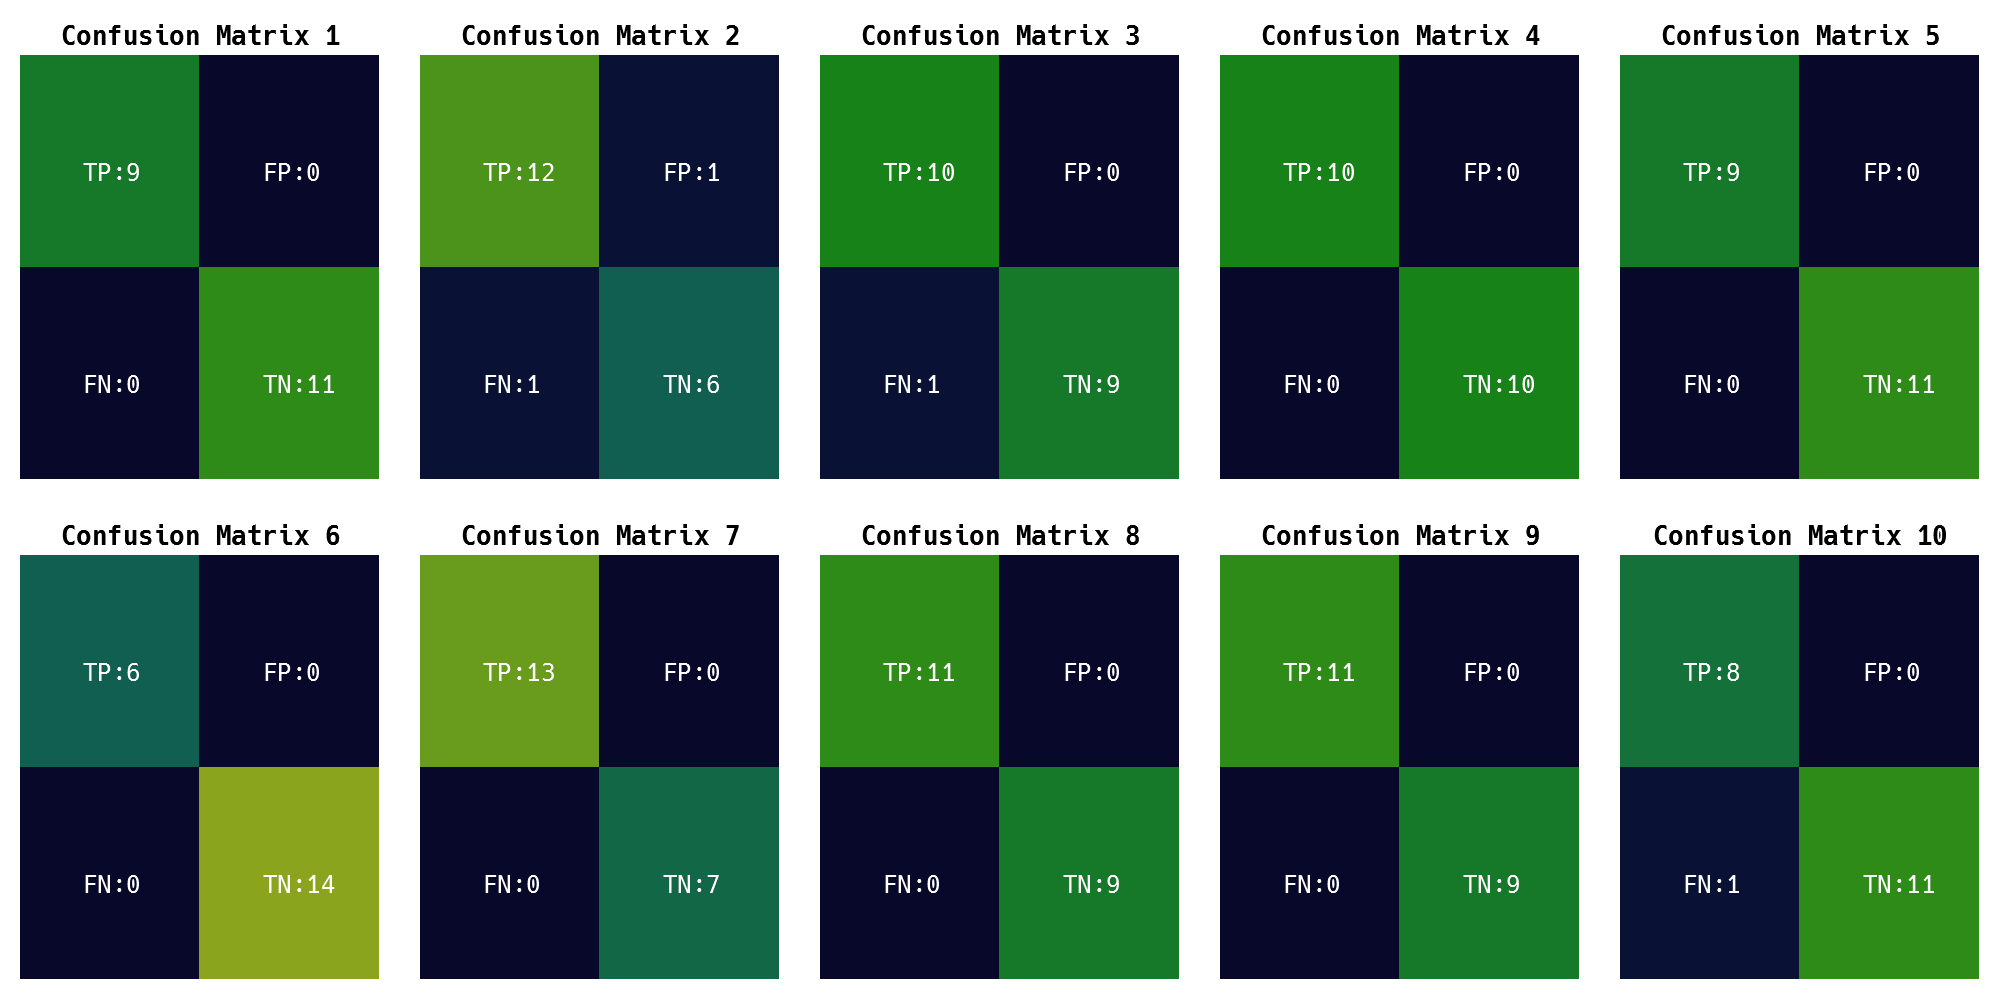
\includegraphics[width=0.9\textwidth]{cross-2-8-1/confusion_matrix}
		\caption{Each iterations validation set confusion matrix where y-axis is an actual class $1, 0$ top to bottom and x-axis is predicted class $1, 0$ left to right.}
	\end{subfigure}
	\caption{Training result of Cross-2-4-1.}
	\label{fig:10}
\end{figure}
\FloatBarrier

\subsection*{Analysis}
From \cref{table:2}, we can see that

\begin{table}[htp]
	\resizebox{\textwidth}{!}{%
		\begin{tabular}{|l|c|c|c|c|}
			\hline
			                                                                 & Cross-2-4-1  & \begin{tabular}[c]{@{}c@{}}Cross-2-4-1\\ with no momentum\end{tabular} & \begin{tabular}[c]{@{}c@{}}Cross-2-4-1\\ with small learning rate\end{tabular} & Cross-2-8-1    \\ \hline
			Training Time (seconds)                                          & \textbf{121} & 123                                                                    & 122                                                                            & 218            \\ \hline
			\begin{tabular}[c]{@{}l@{}}Validation Mean Accuracy\end{tabular} & 0.915        & 0.810                                                                  & 0.795                                                                          & \textbf{0.970} \\ \hline
		\end{tabular}%
	}
	\caption{Training time and validation mean accuracy (blue line on (a) \cref{fig:7} - \cref{fig:10}) of each Flood network}
	\label{table:2}
\end{table}
\end{document}
